
%%%%%%%%%%%%%%%%%%%%%%%%%%%%%%%%%%%%
%						Deep Neural Network 
%
%	 Author: Valgi0
%
%  Goal: All notes from various sources 
% 
%%%%%%%%%%%%%

\documentclass[12pt,a4paper,twoside,openright]{scrbook}

\usepackage[utf8]{inputenc}
\usepackage[english]{babel}
\usepackage[T1]{fontenc}


\usepackage{amsmath,amsfonts,amssymb,amsthm}
\usepackage{caption}
\usepackage[usenames]{color}
\usepackage{enumerate}
\usepackage{fancyhdr}
\usepackage{fancyvrb}
\usepackage{float}
\usepackage{graphicx}
\usepackage{booktabs}
\usepackage{indentfirst}
\usepackage{listings}
\usepackage{marvosym}
\usepackage{multicol}
\usepackage{sectsty}
\usepackage{subcaption}
\usepackage{tocloft}
\usepackage{microtype}
\usepackage[table]{xcolor}
\usepackage{url}
\usepackage{hyperref}
\usepackage{adjustbox}
\usepackage{blindtext}


\hypersetup{%
	pdfpagemode={UseOutlines},
	bookmarksopen,
	pdfstartview={FitH},
	colorlinks,
	linkcolor={black},
	citecolor={black},
	urlcolor={black}
}


\makeindex

\subject{my note about}
\title{Basic (and Maybe advanced) Deep Learning stuff }
\subtitle{theory and samples}
\author{Valgi0 (me as always)}

\begin{document}

\frontmatter 

\maketitle


\newpage

\tableofcontents

\newpage

\listoffigures

\mainmatter

\pagestyle{fancy} 
\fancyhead[LO]{\nouppercase{\rightmark}}
\fancyhead[RE]{\nouppercase{\leftmark}}
\fancyhead[LE,RO]{\thepage}
\fancyfoot{}

%% CAPITOLO 1
\chapter{Why this documents}
I feel the exigence to put together all my notes and my experience in this wide word of Deep Neural Network. I want them in one place with a good organization allowing me and the reader to access to what I need quickly. This thought came to my mind while I was working to my dissertation thesis, and for the haste, I used to write notes every where and when I needed them they were hard to find. Btw I don't care to write why I'm doing this so

\section{Where Information come from}
I'm going to use some books freely distributed and one day I'll put the links here. Stay tuned

\section{Chapters organization}
Each chapter contains arguments to one topic and information are organized following this schema:
\begin{itemize}
\item Introduction to the topic
\item Theory about topic
\item Examples maybe
\item Related links or papers ( Idk )
\end{itemize}

\section{Notation}
\begin{itemize}
\item \textit{a,b,c} are scalars
\item \textbf{a,b,c} are vectors
\item \textbf{A,B,C} are matrices
\end{itemize}


\chapter{Let's start}

In this chapter we are going to see the very basic of Neural Network like \textit{Neurons}, \textit{Links}, \ldots.

\section{Single Neuron}
Neuron is the basic unit of Neural Network and is just a mathematical function applied to an input.
Let's define an input a scalar \textit{i} a scalar weight \textit{w}, a scalar bias \textit{b} and a function \textit{f}.
Neuron function is:
\begin{equation}
a = f(iw + b)
\end{equation}
Function \textit{f} is called \textbf{Activation Function} or sometimes \textbf{Transfer function} and usually is a non linear function.

\subsection{Example of neuron}
\textit{i} = 5, \textit{w} = 0.5, \textit{b} = 2 and \textit{f(x)} = $x + 1$  
\begin{equation}
f(5*0.5 + 2) = f(4,5) = 5.5
\end{equation}

\section{Transfer functions}
\begin{figure}
    \centering
    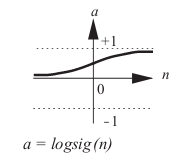
\includegraphics[scale=0.65]{img/log-sigmoid-function.png}
    \caption{log-sigmoid function}
    \label{img:log-sigmoid}
\end{figure}{}
Or Activation function are chosen during model creation in fact they are Hyper-Parameters. They can be linear or non-linear. Now some of the most important linear functions are listed:
\begin{itemize}
\item \textbf{Hard Limit Transfer Function}. This function produce 0 if input value is negative or 1 if value is equal or greater that 0. It creates a step and it is used for binary classification problems
\item \textbf{Linear Function}. $f(x) = x*m +q$. It is the function of the line.
\item \textbf{log-sigmoid transfer function}. $f(x) = \frac{1}{1+e^{-x}}$. This function produce a value always positive and you can see the graphic at the figure \ref{img:log-sigmoid}
\end{itemize}
\begin{figure}
    \centering
    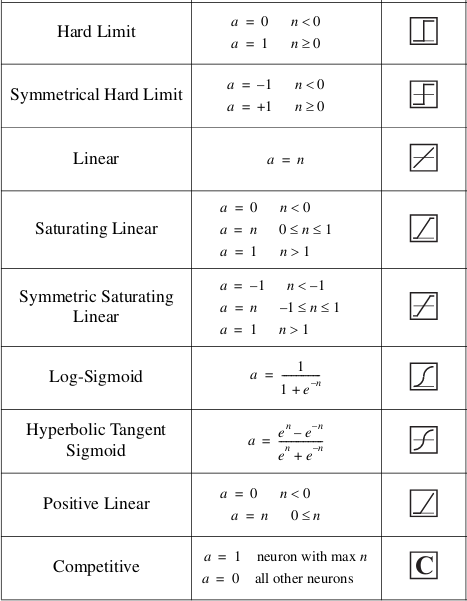
\includegraphics[scale=0.65]{img/activation-functions-table.png}
    \caption{Overview of basic activation functions}
    \label{img:activation-functions-basic}
\end{figure}


\section{Multi-input Neuron}
Usually neuron has more than one input at time. Each of them want a private \textit{w} while \textit{b} the bias is one for all. Under this light we can say that input \textbf{i} is a column vector of $i_0,.., i_n$ elements and neuron contains a scalar \textit{b} and a vectors of \textbf{w} of n weights. Using \textit{f} as linear function $f(x) =x + 1$ the neuron perform this equation:
\begin{equation}
a = f(\textbf{wi} + b) = f((\sum_{j=0}^{n} w_j * i_j) + b)
\end{equation}

\subsection{Example}
\textbf{i} = $5,6,7$ \textbf{w} = $1,2,-1$ \textit{b} = 2 and \textit{f(x)} = $x + 1$  
\begin{equation}
f(5*1 + 6*2 + 7*-1 + 2) = f(12) = 13
\end{equation}

\section{Multi-neurons}
Often Input vector goes to multiple neurons and these neurons are a Layer. It is important keep in mind that:
\begin{itemize}
\item All Neurons take all input. So \textit{w} weights is a vector with the same dimension of the input vector
\item All Neuron produce a scalar so the number of neurons in a layer is the number of  outputs.
\item Each neuron has its bias so a layer has a vector of bias one per neurons 
\end{itemize}

Let's define input \textbf{i} a column vector and weight \textbf{W} as a matrix $m*n$ where $m$ is the number of the neuron and $n$ the number of the input elements in \textbf{i}. \textit{f} is the activation function:

\begin{equation}
\textbf{a} = f(\textbf{W}\textbf{i} + b)
\end{equation}

From the above equation we can see that a matmul is performed between weights matrix and input column vector. So row $j$, that is the weight vector of the neuron $j$ is multiplied and summed with the whole input column vector.

\begin{equation}
  \begin{bmatrix}
w_{0,0} & w_{0,1} & \ldots & w_{0,n} \\
w_{1,0} & w_{1,0} & \ldots & w_{1,n} \\
\vdots & \vdots & \vdots & \vdots \\
w_{m,0} & w_{m,1} & \ldots & w_{m,n} \\
  \end{bmatrix} * \begin{bmatrix}
  i_0 \\ i_1 \\ \vdots \\ i_n
  \end{bmatrix}
\end{equation}

So a neural layer can be seen as a matrix of weight and a Bias vector:
\begin{equation}
Layer_w = \begin{bmatrix}
n_0 \\ n_1\\ n_2\\ \vdots \\ n_m
\end{bmatrix} = \begin{bmatrix}
w_{0,0} & w_{0,1} & \ldots & w_{0,n} \\
w_{1,0} & w_{1,0} & \ldots & w_{1,n} \\
\vdots & \vdots & \vdots & \vdots \\
w_{m,0} & w_{m,1} & \ldots & w_{m,n} \\
\end{bmatrix}
\end{equation}
\begin{equation}
Layer_b = [b_0, b_1, b_2, \ldots , b_m]
\end{equation}

Mathematically a layer can be represents just by \textbf{W} the weight matrix and \textbf{b} the bias vector.

\section{Multi Layers}

A neural network has more layers. The first layer is called \textbf{Input layer} the last in called \textbf{Output layer} and the ones in the middle are \textbf{Hidden Layers}. 
Each layers can have different number of neurons and different activation function. So a basic multi-layer network with $l$ layers is defined by $f_0, ..., f_l$ activation functions, $\textbf{W}_0,..., \textbf{W}_l$ weight matrices and $\textbf{b}_0,...,\textbf{b}_l$ or just \textbf{B} bias (matrix contains in row $j$ the bias vector for the layer $j$).
This network take inputs with the first layer, generate output and then gives this output to the second layer and so on.
A Multi layer Network performs:
\begin{equation}
\textbf{a} = f_l(f_{l-1}(\ldots * \textbf{W}_{l-1} + \textbf{b}_{l-1}) * \textbf{W}_{l} + \textbf{b}_{l})
\end{equation}

This Multi-layer neural Network is called \textbf{Feed Forward Neural Network}

\section{Recurrent Neural Network}
Feed forward neural network has layers and layer has neurons. Each Neuron take a input vector \textbf{i} and produce a scalar \textit{a}. Differently, Recurrent Neural Network takes two input vector the input vector \textbf{i} and some \textit{a'} that is the output of the previous input. Let's imagine we have a time series of data $i_0,...,i_t$. This data must be given to the model respecting the sequence but we want model somehow remember previous data. For this kind of task Recurrent Neural Network was created. They have layers and neurons but each neuron has two vectors and a bias: \textit{u} weights for the input, \textit{w} weights for its layer output at the previous step and \textit{b} the bias. Let me explain in a intuitive way before using math: the input is a series of vectors. First vector $i_0$ is taken and is given to the first layer of the model. Each neurons of this layer get the input vector $i_0$ and produce a scalar $a_0$ and with other neurons output of that layer it creates the layer output \textit{a}  Nothing new until now. Output goes to the second layer and so on until last layer. Second input is taken $i_1$ and neuron  receives it and the previous layer output \textit{a}. Using both of them it compute the next scalar output $nexta_0$. And so on! 

Let's define its behavior using some cool math. Our network is composed by 1 layer with 1 neuron:
%\begin{equation}
%  inputsequence=\textbf{i_0}, \ldots ,\textbf{i_k} \\
%  f_{neuron} = ActivationFunc( b + \textbf{w}*a'_{t - 1} + \textbf{u}*\textbf{i_t}) = a_{t}
%\end{equation}
The neuron takes at time t in input $a'_{0,t - 1}$ and $i_{0,t}$ and produce $a_{t}$. In this case with just one neuron the layer output coincide with the neuron output. After that the following equation is performed to compute $a'_t$
\begin{equation}
a'_t = c + \textbf{v}a_t
\end{equation}

Let's imagine to have a Recurrent Neural Network with more layers and more neurons for each layers. The above equations become:
\begin{equation}
\textbf{a_t} = ActivationFunc(\textbf{b} + \textbf{W}*\textbf{a'_{l,t-1} + \textbf{U}*\textbf{i_t}
\end{equation}
$a'_{l,t-1}$ means the column vector output from the layer $l$ at time step $t-1$
\begin{equation}
\textbf{a'_{l,t}} = \textbf{c} + \textbf{V}\textbf{a_{l,t}} 
\end{equation} 






\end{document}
